\documentclass[11pt]{article}
\usepackage[margin=1in]{geometry}
\usepackage{amsmath,amssymb,amsthm,amscd,mathtools}
\usepackage{graphicx}
\usepackage[hidelinks]{hyperref}
\usepackage{microtype}

\newtheorem{theorem}{Theorem}
\newtheorem{lemma}{Lemma}
\newcommand{\R}{\mathbb R}
\newcommand{\Espace}{\mathcal E}
\newcommand{\Fspace}{\mathcal F}
\newcommand{\ConeE}{\mathcal C}
\newcommand{\ConeF}{\mathcal D}
\newcommand{\tp}{\widehat\otimes_\pi}
\newcommand{\te}{\widehat\otimes_\varepsilon}
\DeclareMathOperator{\lin}{lin}

\title{A counterexample to completed projective-cone semisimplicity}
\author{Candidate counterexample packet for arXiv:2009.11843}
\date{19 July 2026}

\begin{document}
\maketitle

\paragraph{Status.}
\texttt{candidate counterexample -- likely valid}.  The theorem below gives a full negative answer to Question 5.16 (labelled \texttt{q:completed-semisimple} in the source) of van Dobben de Bruyn's memoir \cite{source}.

\section{Source question}

The source asks whether, for real Banach spaces $E,F$ with closed proper cones $E_+,F_+$, the completed projective cone in $E\tp F$ must be contained in a closed proper cone.  Equivalently, must the continuous bilinear forms that are nonnegative on $E_+\times F_+$ separate points of $E\tp F$?

\begin{center}
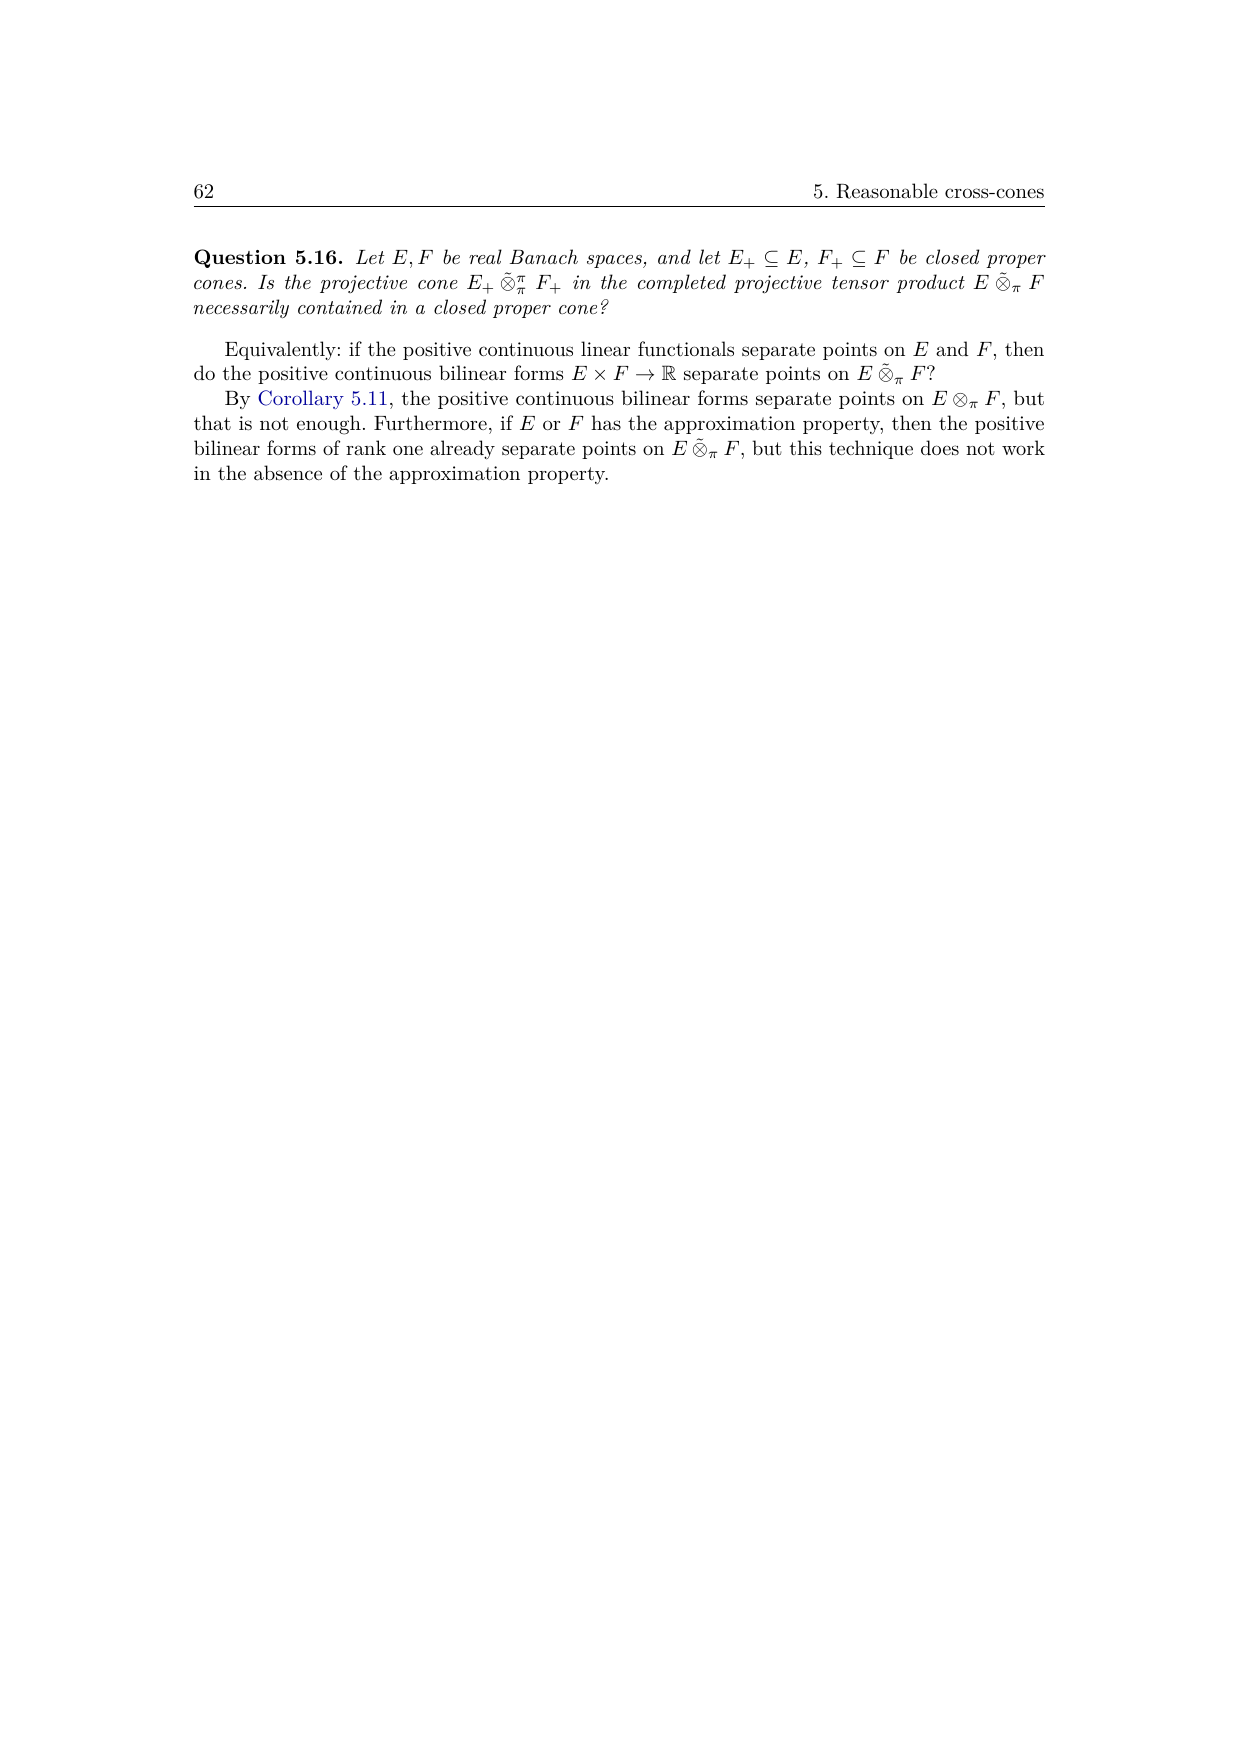
\includegraphics[width=\textwidth,trim=0 570 0 50,clip]{figures/source_question.png}
\end{center}

\section{Idea of the proof}

The source observes that the canonical map from a completed projective tensor product to the corresponding injective tensor product need not be injective, but leaves open whether the projective cone can nevertheless remain semisimple.  The key idea is to use a nonzero tensor in precisely such a kernel, together with cones whose gauges come from injective maps into Hilbert space.  Positivity on four signed boundary pairs forces every positive bilinear form to factor, on the relevant tensor coordinates, through the two Hilbert spaces.  The kernel tensor is therefore annihilated by every positive functional.  Cone bipolarity puts both signs of its nonzero embedded image in the closed projective cone.  The constructed base cones are nevertheless closed, proper, and generating, so they satisfy the source hypotheses while their completed projective cone violates the asserted conclusion.

\section{Statement}

\begin{theorem}\label{thm:main}
There exist separable real Banach spaces $\Espace,\Fspace$ and closed, proper, generating cones $\ConeE\subseteq\Espace$, $\ConeF\subseteq\Fspace$ such that the closed projective cone
\[
 \overline{\operatorname{cone}}\{u\otimes v:u\in\ConeE,\ v\in\ConeF\}
 \subseteq \Espace\tp\Fspace
\]
has nonzero lineality.  Consequently it is not contained in any proper cone.  In particular, the answer to Question 5.16 of \cite{source} is negative.
\end{theorem}

\section{Ingredients}

We use the classical fact that there are real Banach spaces $X,Y$ for which the canonical contraction
\begin{equation}\label{eq:kappa}
 \kappa_{X,Y}:X\tp Y\longrightarrow X\te Y
\end{equation}
is not injective.  This is the standard tensor formulation of failure of the approximation property; the source itself recalls this fact immediately before posing its question, referring to \cite[Theorem 5.6]{defantfloret}.  We may take $X,Y$ separable.  Indeed, start with a nonzero $z\in\ker\kappa_{X,Y}$, choose an absolutely convergent projective representation of $z$, and replace $X,Y$ by the closed spans of the countably many vectors in that representation.  The resulting tensor is still nonzero (its image in the original projective tensor product is $z$), while injectivity of the injective tensor norm on subspaces shows that it still maps to zero.

Every separable real Banach space $X$ admits a bounded injective linear map into a real Hilbert space.  To see this, choose a sequence $(f_m)\subseteq B_{X^*}$ that separates points and set
\[
 Jx=(2^{-m/2}f_m(x))_{m\ge1}\in\ell_2.
\]
Then $\|J\|\le1$ and $J$ is injective.  Apply this to $X,Y$, obtaining bounded injections
\[
 J:X\to H,\qquad K:Y\to L
\]
into real Hilbert spaces.  We replace $H,L$ by the closures of the respective ranges and define the continuous norms
\[
 p(x)=\|Jx\|_H,\qquad q(y)=\|Ky\|_L.
\]
These are genuine norms, though generally not equivalent to the original Banach norms.

\begin{lemma}\label{lem:hilbert-kernel}
If $z\in\ker\kappa_{X,Y}$, then its image under
\[
 J\otimes K:X\tp Y\longrightarrow H\tp L
\]
is zero.
\end{lemma}

\begin{proof}
Functoriality gives the commutative diagram
\[
\begin{CD}
X\tp Y @>{J\otimes K}>> H\tp L\\
@V{\kappa_{X,Y}}VV @VV{\kappa_{H,L}}V\\
X\te Y @>{J\otimes K}>> H\te L.
\end{CD}
\]
The lower route sends $z$ to zero.  Since Hilbert spaces have the approximation property, $\kappa_{H,L}$ is injective.  Hence the upper image of $z$ is zero.
\end{proof}

\section{Construction of the cones}

Equip
\[
 \Espace=\R\oplus_1X,\qquad \Fspace=\R\oplus_1Y
\]
with their usual sum norms, and define
\begin{equation}\label{eq:cones}
 \ConeE=\{(t,x):t\ge p(x)\},\qquad
 \ConeF=\{(s,y):s\ge q(y)\}.
\end{equation}
Both cones are closed because $p,q$ are continuous.  They are proper: if $(t,x)$ and $-(t,x)$ both belong to $\ConeE$, then $t\ge p(x)$ and $-t\ge p(x)$, whence $t=0$ and $x=0$; similarly for $\ConeF$.  They are also generating.  For example, with $r=p(x)+|t|$,
\[
 (t,x)=(r+t,x)-(r,0),
\]
and both terms on the right belong to $\ConeE$.

The following four-sign estimate is the core of the counterexample.

\begin{lemma}\label{lem:positive-factor}
Let $B:\Espace\times\Fspace\to\R$ be a continuous bilinear form that is nonnegative on $\ConeE\times\ConeF$.  Write uniquely
\begin{equation}\label{eq:decomposeB}
 B((t,x),(s,y))=a ts+s f(x)+t g(y)+A(x,y),
\end{equation}
where $a\in\R$, $f\in X^*$, $g\in Y^*$, and $A:X\times Y\to\R$ is continuous bilinear.  Then $a\ge0$ and
\begin{equation}\label{eq:domination}
 |A(x,y)|\le a\,p(x)q(y)\qquad(x\in X,\ y\in Y).
\end{equation}
Consequently $A$ extends to a continuous bilinear form $\widetilde A:H\times L\to\R$.
\end{lemma}

\begin{proof}
Since $(1,0)$ belongs to each cone, positivity gives $a\ge0$.  Fix $x\in X$ and $y\in Y$, and abbreviate $P=p(x)$ and $Q=q(y)$.  For every $\sigma,\tau\in\{-1,1\}$, the vectors $(P,\sigma x)$ and $(Q,\tau y)$ belong to the respective cones.  Thus
\[
 aPQ+\sigma Qf(x)+\tau Pg(y)+\sigma\tau A(x,y)\ge0.
\]
Adding the inequalities for $(\sigma,\tau)=(1,1)$ and $(-1,-1)$ yields $A(x,y)\ge-aPQ$.  Adding those for $(1,-1)$ and $(-1,1)$ yields $A(x,y)\le aPQ$.  This is \eqref{eq:domination}.  Hence
\[
 |A(x,y)|\le a\|Jx\|_H\|Ky\|_L,
\]
so $A$ descends to the dense ranges $JX\subseteq H$, $KY\subseteq L$ and extends continuously to $H\times L$.
\end{proof}

\section{Proof of the counterexample}

\begin{proof}[Proof of Theorem \ref{thm:main}]
Choose $0\ne z\in\ker\kappa_{X,Y}$.  Let $\iota_X:X\to\Espace$ and $\iota_Y:Y\to\Fspace$ be the coordinate inclusions $x\mapsto(0,x)$ and $y\mapsto(0,y)$, and put
\[
 w=(\iota_X\otimes\iota_Y)z\in\Espace\tp\Fspace.
\]
The coordinate projections $\Espace\to X$ and $\Fspace\to Y$ give a bounded left inverse on the projective tensor products, so $w\ne0$.

Let $B$ be any continuous bilinear form nonnegative on $\ConeE\times\ConeF$, and decompose it as in \eqref{eq:decomposeB}.  Its value on $w$ is $A(z)$.  Lemma \ref{lem:positive-factor} factors $A$ through $H\times L$, while Lemma \ref{lem:hilbert-kernel} says that the image of $z$ in $H\tp L$ is zero.  Therefore
\begin{equation}\label{eq:annihilate}
 B(w)=A(z)=0
\end{equation}
for every positive continuous bilinear form $B$.

Let
\[
 \mathcal K=\overline{\operatorname{cone}}\{u\otimes v:u\in\ConeE,\ v\in\ConeF\}
 \subseteq\Espace\tp\Fspace.
\]
The dual cone $\mathcal K^*$ consists exactly of the continuous bilinear forms nonnegative on $\ConeE\times\ConeF$.  Equation \eqref{eq:annihilate} says that every element of $\mathcal K^*$ vanishes on $w$.  By the bipolar theorem for closed convex cones,
\[
 \mathcal K=\{v:B(v)\ge0\text{ for every }B\in\mathcal K^*\}.
\]
Both $w$ and $-w$ therefore belong to $\mathcal K$.  Since $w\ne0$, the lineality space $\mathcal K\cap(-\mathcal K)$ is nonzero.  Any cone containing $\mathcal K$ contains both $w$ and $-w$, and hence cannot be proper.  This proves the theorem.
\end{proof}

\section{Verification and scope}

The proof uses only four standard inputs: existence of a noninjective projective-to-injective tensor map, bounded Hilbert-space injections for separable Banach spaces, injectivity of that tensor map for Hilbert spaces, and the bipolar theorem.  The new step is the cone construction \eqref{eq:cones} and the four-sign domination \eqref{eq:domination}.

The cones in the counterexample are stronger than requested: they are generating as well as closed and proper.  No explicit classical model of a Banach space without the approximation property is needed; any standard noninjective pair supplies the construction.

For human review, the highest-value checks are the projective/injective commuting diagram and separable reduction, followed by the four-sign cancellation and the final bipolar step; the accompanying \texttt{verification\_report.md} audits these points individually.

\section{Novelty-check status}

The run's lightweight registry, solution, and attempt indexes had no record for arXiv:2009.11843 or Question 5.16.  A bounded search on 19 July 2026 used the arXiv identifier, title, author, source label \texttt{q:completed-semisimple}, the exact question phrase ``necessarily contained in a closed proper cone'', and the core terms ``completed projective cone'' and ``positive bilinear forms separate points''.  Current source and exact-phrase results contained no claimed resolution; the author's 2023 thesis repeats the question as open.  This bounded search does not certify novelty.

\begin{thebibliography}{9}
\bibitem{source}
J. van Dobben de Bruyn,
\emph{Tensor Products of Convex Cones},
arXiv:2009.11843 (2020), Question 5.16.

\bibitem{defantfloret}
A. Defant and K. Floret,
\emph{Tensor Norms and Operator Ideals},
North-Holland Mathematics Studies 176, 1993.
\end{thebibliography}

\end{document}
